\section{Compression, Prediction and Lossless Coding}


\begin{questionbox}{Domanda 5}
Principles of image compression. Discuss the criteria for evaluating a compression algorithm: rate, quality, [Bonus: robustness, delay, complexity].
\end{questionbox}


\begin{itemize}
  \item \textbf{Compression exploits}:
  \begin{itemize}
    \item \textbf{statistical redundancy} $\rightarrow$ correlated samples/blocks/frames;
    \item \textbf{spatial / temporal redundancy} $\rightarrow$ repeated structures;
    \item \textbf{psychovisual redundancy} $\rightarrow$ imperceptible distortion.
  \end{itemize}
  \item \textbf{Types}:
  \begin{itemize}
    \item \textbf{lossless} $\rightarrow$ exact reconstruction, lower compression;
    \item \textbf{lossy} $\rightarrow$ approximate but perceptually close reconstruction, higher compression.
  \end{itemize}
  \item \textbf{Rate}:

\end{itemize}
$$
R_{\text{image}} = \frac{B_{\text{out}}}{NM} \quad [\text{bpp}]
$$

$$
R_{\text{stream}} = \frac{B_{\text{out}}}{T} \quad [\text{bit/s}]
$$

\begin{itemize}
  \item \textbf{Compression ratio}:

\end{itemize}
$$
\text{CR} = \frac{B_{\text{in}}}{B_{\text{out}}}
$$

\begin{itemize}
  \item \textbf{Distortion / quality}:

\end{itemize}
$$
D(f,\hat{f}) = \frac{1}{NM}\|f-\hat{f}\|^2
$$

$$
\text{PSNR}(f,\hat{f}) = 10\log_{10}\left(\frac{V^2}{D(f,\hat{f})}\right)
$$

\begin{itemize}
  \item \textbf{Perceptual weighting}:

\end{itemize}
$$
D_W(f,\hat{f}) = \frac{1}{NM}\|h \star (f-\hat{f})\|^2
$$

$$
\text{WPSNR}(f,\hat{f}) = 10\log_{10}\left(\frac{V^2}{D_W(f,\hat{f})}\right)
$$

\begin{itemize}
  \item \textbf{Tradeoffs} $\rightarrow$ rate, quality, robustness, delay, complexity; also SSIM, LPIPS.

\end{itemize}
\begin{questionbox}{Domanda 6}
A zero-mean Gaussian random signal has an autocorrelation function:

$$
r_X(n-m)=E[X(n)X(m)] = \sigma^2\rho^{|n-m|}
$$

\begin{itemize}
  \item Consider the predictor $V(n)=X(n-1)$. For which values is the prediction gain positive?
  \item Optimal linear predictor is $V(n)=-\sum_{i=1}^{P} a_i x_{n-i}$, with $a=-R_X^{-1}r$, $R_X(i,j)=r_X(i-j)$, $r=[r_X(1)\cdots r_X(P)]^T$. Find optimal linear predictor of order $P=1$ and compute prediction gain, compare then with previous case.
  \item Compute the optimal predictor of order 2. Compare with the previous cases.
\end{itemize}
\end{questionbox}


\textbf{Given}:

$$
r_X(n-m)=\mathbb{E}[X(n)X(m)] = \sigma^2\rho^{|n-m|}
$$

\begin{itemize}
  \item Predictor $V(n)=X(n-1)$:

\end{itemize}
$$
\sigma_y^2 = \mathbb{E}[(X(n)-X(n-1))^2] = 2\sigma^2(1-\rho)
$$

$$
G_P = 10\log_{10}\left(\frac{1}{2(1-\rho)}\right)
$$

\begin{itemize}
  \item \textbf{Positive gain if and only if}:

\end{itemize}
$$
\rho > \frac{1}{2}
$$

\begin{itemize}
  \item \textbf{Optimal linear predictor}:

\end{itemize}
$$
V(n) = -\sum_{i=1}^{P} a_i x(n-i), \quad \vec{a}^{\,opt} = -R_X^{-1}\vec{r}
$$

\begin{itemize}
  \item For $P=1$:

\end{itemize}
$$
a_1^{opt}=-\rho \quad \Rightarrow \quad V(n)=\rho X(n-1)
$$

$$
\sigma_y^2=\sigma^2(1-\rho^2), \quad
G_P = 10\log_{10}\left(\frac{1}{1-\rho^2}\right)
$$

\begin{itemize}
  \item For $P=2$:

\end{itemize}
$$
R_X = \sigma^2
\begin{bmatrix}
1 & \rho \\
\rho & 1
\end{bmatrix},
\quad
\vec{r} = \sigma^2
\begin{bmatrix}
\rho \\
\rho^2
\end{bmatrix}
$$

$$
\vec{a}^{\,opt} =
\begin{bmatrix}
-\rho \\
0
\end{bmatrix}
$$

\begin{itemize}
  \item \textbf{Result} $\rightarrow$ second tap gives no extra gain for AR(1) source.

\end{itemize}
\begin{questionbox}{Domanda 7}
Draw and comment on the schemes of predictive quantization (encoder and decoder).
\end{questionbox}


\begin{figure}[H]
\centering
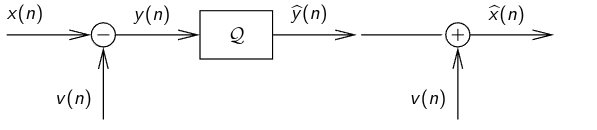
\includegraphics[width=0.75\textwidth]{images/Predictive_quantization_-_open_loop.png}
\caption{Predictive quantization - open loop.png}
\end{figure}

\begin{itemize}
  \item \textbf{Open-loop predictive quantization}:
  \begin{itemize}
    \item subtract predictor $v(n)$ from $x(n)$ $\rightarrow$ residual $y(n)$;
    \item \textbf{quantize residual} $\rightarrow$ $\hat y(n)$;
    \item add $v(n)$ back $\rightarrow$ reconstruction $\hat x(n)$.
  \end{itemize}
  \item \textbf{Problem} $\rightarrow$ encoder predicts from original samples, decoder from reconstructed samples $\rightarrow$ \textbf{drift}.

\end{itemize}
\begin{figure}[H]
\centering
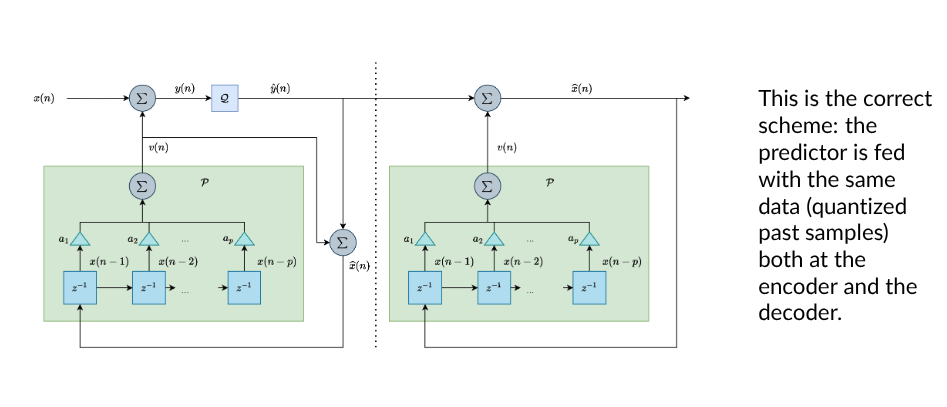
\includegraphics[width=0.75\textwidth]{images/Predictive_quantization_-_correct_closed_loop.png}
\caption{Predictive quantization - correct closed loop.png}
\end{figure}

\begin{itemize}
  \item \textbf{Closed-loop encoder} $\rightarrow$ encoder contains same reconstruction loop as decoder.
  \item \textbf{Predictor input matches both sides}:

\end{itemize}
$$
y(n)=x(n)-v(n), \quad \hat{x}(n)=\hat{y}(n)+v(n)
$$

\begin{itemize}
  \item Useful if and only if residual variance is smaller than original variance.

\end{itemize}
\begin{questionbox}{Domanda 8}
Discuss the principles of lossless coding.
\end{questionbox}


\begin{itemize}
  \item \textbf{Lossless coding} $\rightarrow$ maps symbols to bitstrings; reconstructs original sequence exactly.
  \item \textbf{Alphabet/code}:

\end{itemize}
$$
\mathcal{X}=\{x_1,\dots,x_M\}, \quad
\mathcal{C}: \mathcal{X}\rightarrow \{0,1\}^*
$$

\begin{itemize}
  \item \textbf{Fixed-length coding}:

\end{itemize}
$$
R=\lceil\log_2 M\rceil
$$

\begin{itemize}
  \item \textbf{VLC} $\rightarrow$ probable symbols get shorter codewords:

\end{itemize}
$$
\bar{L} = \sum_i p_i l_i
$$

\begin{itemize}
  \item \textbf{Prefix code} $\rightarrow$ no codeword is prefix of another $\rightarrow$ instantaneous decoding.
  \item \textbf{McMillan theorem} $\rightarrow$ best uniquely decodable code has same performance as best prefix code.
  \item \textbf{Kraft inequality}:

\end{itemize}
$$
\sum_i 2^{-l_i} \le 1
\iff
\text{prefix code exists with lengths } \{l_i\}
$$

\begin{itemize}
  \item \textbf{Entropy lower bound}:

\end{itemize}
$$
H(X)=-\sum_i p_i \log_2 p_i
$$

\begin{itemize}
  \item \textbf{Shannon}:

\end{itemize}
$$
H(X) \le \bar{L} < H(X)+1
$$

\begin{questionbox}{Domanda 9}
Consider a source that emits the symbols A, B, C, D, E, and F. The probabilities of these symbols are given in the following table:

$$
p_A=0.3,\ p_B=0.1,\ p_C=0.05,\ p_D=0.18,\ p_E=0.15,\ p_F=0.22
$$

\begin{itemize}
  \item Describe the Huffman Algorithm.
  \item Compute Huffman code for this distribution.
  \item Compare the average length of the Huffman code with the distribution entropy.
\end{itemize}
\end{questionbox}


\begin{itemize}
  \item \textbf{Huffman algorithm} $\rightarrow$ repeatedly merge two least probable symbols.
  \item \textbf{One optimal code}:
  \begin{itemize}
    \item A, $p=0.30$ $\rightarrow$ `10`, length 2
    \item B, $p=0.10$ $\rightarrow$ `1111`, length 4
    \item C, $p=0.05$ $\rightarrow$ `1110`, length 4
    \item D, $p=0.18$ $\rightarrow$ `00`, length 2
    \item E, $p=0.15$ $\rightarrow$ `110`, length 3
    \item F, $p=0.22$ $\rightarrow$ `01`, length 2

  \end{itemize}
\end{itemize}
$$
\bar{L}=0.30\cdot2+0.10\cdot4+0.05\cdot4+0.18\cdot2+0.15\cdot3+0.22\cdot2 = 2.45
$$

$$
H(X)=-\sum_i p_i\log_2 p_i \approx 2.406 \text{ bit/symbol}
$$

\begin{itemize}
  \item \textbf{Overhead} $\rightarrow$ $\bar{L}-H(X)\approx0.044$ bit/symbol.

\end{itemize}
\begin{questionbox}{Domanda 10}
Why arithmetic encoder is preferred over Huffman for high-performance lossless coding?
\end{questionbox}


\begin{itemize}
  \item \textbf{Huffman} $\rightarrow$ integer codeword lengths $\rightarrow$ penalty for non-dyadic probabilities.
  \item Block Huffman reduces penalty, but alphabet grows as $M^K$.
  \item \textbf{Arithmetic coding} $\rightarrow$ encodes whole sequence as interval in $[0,1)$.
  \item \textbf{Rate}:

\end{itemize}
$$
\mathcal{L} < H(X) + \frac{2}{n}
\xrightarrow[n\to\infty]{}
H(X)
$$

\begin{itemize}
  \item Also suited to adaptive/context probability models.

\end{itemize}
\begin{questionbox}{Domanda 11}
(LLCod) Explain the dif and only iference between Fixed-Length Coding (FLC) and Variable-Length Coding (VLC), and describe why VLC is theoretically superior for non-equiprobable sources.
\end{questionbox}


\begin{itemize}
  \item \textbf{FLC} $\rightarrow$ same codeword length for every symbol; simple, instant parsing, inefficient if probabilities non-uniform.
  \item \textbf{VLC} $\rightarrow$ dif and only iferent lengths; probable symbols shorter.

\end{itemize}
$$
\bar{L} = \sum_i p_i l_i
$$

\begin{itemize}
  \item \textbf{Superiority condition} $\rightarrow$ non-equiprobable source.

\end{itemize}
\begin{questionbox}{Domanda 12}
(LLCod) Discuss the importance of the prefix condition in Variable-Length Coding and how it relates to the concept of instantaneous decodability.
\end{questionbox}


\begin{itemize}
  \item \textbf{Prefix condition} $\rightarrow$ no codeword is prefix of another.
  \item \textbf{Consequence} $\rightarrow$ decoder identifies symbol as soon as codeword ends; no look-ahead.
  \item \textbf{Kraft}:

\end{itemize}
$$
\sum_i 2^{-l_i}\le 1
$$

\begin{itemize}
  \item \textbf{Equality} $\rightarrow$ complete prefix tree.

\end{itemize}
\begin{questionbox}{Domanda 13}
(LLCod) What are the two distinct mechanisms by which “block coding” improves the efficiency of lossless compression?
\end{questionbox}


\begin{enumerate}
  \item \textbf{Sources with memory}:

\end{enumerate}
$$
H(X^K) \le \sum_{i=1}^{K}H(X_i)
$$

$\rightarrow$ dependencies exploited.

\begin{enumerate}
  \item \textbf{Memoryless non-dyadic sources}:

\end{enumerate}
$$
\frac{H(X^K)}{K} \le \frac{L^*}{K} < \frac{H(X^K)}{K} + \frac{1}{K}
$$

$\rightarrow$ integer-length overhead spread over $K$ symbols; overhead/symbol $\rightarrow$ $0$.

\begin{questionbox}{Domanda 14}
(LLCod) Provide a synthetic comparison between the main lossless coding techniques (Exp-Golomb, Huffman, Arithmetic, Dictionary, Neural) in terms of complexity and Latency, and provide a typical use case for each of them.
\end{questionbox}


\begin{itemize}
  \item \textbf{Exp-Golomb}: good for small integers; very low complexity/latency $\rightarrow$ syntax elements, motion-vector residuals.
  \item \textbf{Huffman}: optimal among symbol prefix codes; low/medium complexity, very low latency $\rightarrow$ JPEG, DEFLATE-style coding.
  \item \textbf{Arithmetic}: near entropy; high complexity, medium latency $\rightarrow$ CABAC, context-adaptive coding.
  \item \textbf{Dictionary (LZ/LZW)}: universal for repeated patterns; medium complexity, low/medium latency $\rightarrow$ text, GIF, ZIP-like systems.
  \item \textbf{Neural lossless}: potentially very high efficiency; very high complexity/latency $\rightarrow$ research, high-resolution image models.

\end{itemize}
\begin{questionbox}{Domanda 15}
(LLCod) Describe the principle of the Huffman coding. For the following probability distribution, compute the optimal lossless code, and compare its average length to the source’s entropy:

$$
p_A=0.35,\ p_B=0.1,\ p_C=0.07,\ p_D=0.08,\ p_E=0.12,\ p_F=0.28
$$
\end{questionbox}


\begin{itemize}
  \item \textbf{One optimal Huffman code}:
  \begin{itemize}
    \item A, $p=0.35$ $\rightarrow$ `00`, length 2
    \item B, $p=0.10$ $\rightarrow$ `100`, length 3
    \item C, $p=0.07$ $\rightarrow$ `101`, length 3
    \item D, $p=0.08$ $\rightarrow$ `110`, length 3
    \item E, $p=0.12$ $\rightarrow$ `111`, length 3
    \item F, $p=0.28$ $\rightarrow$ `01`, length 2
  \end{itemize}
  \item \textbf{Relevant lengths}:

\end{itemize}
$$
l_A=l_F=2,\quad l_B=l_C=l_D=l_E=3
$$

$$
\bar{L}=0.35\cdot2+0.28\cdot2+(0.10+0.07+0.08+0.12)\cdot3=2.37
$$

$$
H(X)\approx 2.304 \text{ bit/symbol}
$$

\begin{itemize}
  \item \textbf{Overhead} $\rightarrow$ $\bar{L}-H(X)\approx0.066$ bit/symbol.

\end{itemize}
\begin{questionbox}{Domanda 16}
(LLCod) Which of the following statements best describes the behavior of the Shannon entropy $H(X)$ for a binary random variable with probability $p$?
\end{questionbox}


For $X\sim\text{Bernoulli}(p)$:

$$
H(X)=-p\log_2 p -(1-p)\log_2(1-p)
$$

\begin{itemize}
  \item $H(X)=0$ for $p=0$ or $p=1$.
  \item Maximum at $p=\frac12$:

\end{itemize}
$$
H\left(\frac{1}{2}\right)=1 \text{ bit}
$$

\begin{questionbox}{Domanda 17}
(LLCod) Why is Lempel-Ziv (e.g., LZW) considered a “universal” coding algorithm?
\end{questionbox}


\begin{itemize}
  \item No prior source probability distribution needed.
  \item Encoder and decoder build same dictionary adaptively from observed sequence.
  \item \textbf{Stationary ergodic sources} $\rightarrow$ asymptotically optimal.

\end{itemize}
---

